\chapter{Вопрос-Ответ}

\section{Первый}

\begin{figure}[h!tb] 
	\centering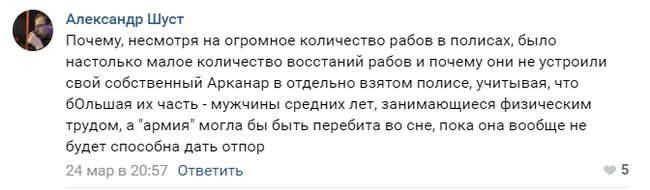
\includegraphics[scale=0.3]{VoprosOtvet/1585473124128666065.png}
	%	\label{fig:scipion} % Unique label used for referencing the figure in-text\end{document}
	%	%\addcontentsline{toc}{figure}{Figure \ref{fig:placeholder}} % Uncomment to add the figure to the table of contents%----------------------------------------------------------------------------------------
	\caption{Вопрос}%	CHAPTER 2
\end{figure}	

Интересный вопрос. Рабство в античности это очень серьезный бизнес, чуть ли не основной для рабовладельческого строя. Поэтому вся нужная инфраструктура для поддержания поголовья рабов в порядке и покорности была выстроена и отлажена также очень и очень давно. Там было всё что нужно:


1. Общество само по себе было заточено под то что ты при определенных вводных мог стать рабом (долговая яма или военное поражение), и жить дальше с урезанными правами. Тоесть то что для нас дичь, для них было печально, но в рамках, рабы - органическая часть социума.


2. Так как индустрии к тому моменту сотни лет, то там отлично понимали как сделать так, чтобы твои предметы не бунтовали. Смешивание, например. Как правило, диаспорами никого не забирали, рабов старались миксовать так, чтобы они не могли даже поговорить ни с кем на своем родном языке. Психологическая ломка и дрессировка. Всякие пряники за послушание. С теми кто выходил из под контроля жестоко и показательно расправлялись.


3. Ну и это жизнь, какая-никакая. Рабом ты тоже мог сделать карьеру, освоить нужные навыки и стать высокооплачиваемым специалистом, жить кучеряво. А свобода... да кому она нужна, они все равно не понимали че с ней делать. Свободу, кстати, тоже можно было получить, став вольноотпущенником. Можно было завести семью, дать образование детям, крч, всякие мещанские вещи для городских рабов вполне присутствовали. Сельским, которые на полях пашут, посложнее канешн, но и там были свои плюсы. А уж если ты раб в небольшом хозяйстве, то ты, считай, член семьи, и относятся к тебе как к быку или собаке, вполне дружелюбно, ценят и заботятся.


В общем, поэтому оно работало вообще, это был веками отлаженный процесс. И вспышки первого века, самыми яркими из которых были два восстания в Сицилии и Спартак, они именно эксцессы, это исключение а не правило. Связанное с двумя факторами. Рабы в Рим перед этими восстаниями поступали сотнями тысяч, цены на них были низкими, и их уровень жизни очень сильно упал, относительно более ранних времен. Настолько упал, что жизнь их превратилась из достаточно приемлемой в невыносимую. Второе это то, что по большей части крупные единовременные поступления рабского поголовья были после военных побед, и в рабство обращали пленных. А это вооруженные и озлобленные люди, ломать их психологически куда труднее, чем каких-нибудь пейзан.


Но даже эти два фактора накаляли обстановку, но не более того. А затем что-то происходило, что-то крайне тупое и со стороны самих римлян. Рвется там где тонко, вот оно и рвалось, и начинался кровавый хаос, который римляне сначала не могли удержать под контролем (из-за большого количества горючего материала), но потом неизбежно очухивались и топили их в крови. Причем яб даже не сказал что это было опасно для государства, так как в первую очередь Рим на отличненько восстание локализовывал, и не давал ему разрастаться как снежный ком. А потом лучшая военная машина античности принималась за проблему, и с нарастающим усилием её давила. При этом ни разу оно не вышло из под контроля настолько, чтобы сильно паниковать.

Даже со Спартаком римляне фактически справились силами итальянского ополчения, которое организовывал один единственный олигарх, Марк Красс, хоть и с широкими полномочиями. При этом к концу, когда Красс уже заканчивал, прибыл Помпей из Испании, где как раз с Серторием покончили. С ним была армия испанских ветеранов, только что закончивших шестилетнюю войну в горах. Это я к тому, что еслиб Красс не шмог, то Помпей бы точно закончил. А еслиб не смог и он, хотя это фантастика, то из Азии можно было снять армии Лукулла, и перебросить в Италию. Крч, Рим даже не сильно напрягался, хотя это, канешно, финансовые и людские потери, очень неприятно. Но для Республики не опасно.


Однако выводы были сделаны, и больше скопления такого количества горючего материала в одном месте не допускали. Например, как раз после Спартака начали массовый перенос производств из Италии в Африку, там и климат получше и потише. А потом, уже при Цезаре, вообще гайки подраскрутили, что в итого, при Августе, выльется для рабов в колонат, тоесть де-факто в крепостное право.

Такие дела.

\section{Второй}

\begin{figure}[h!tb] 
	\centering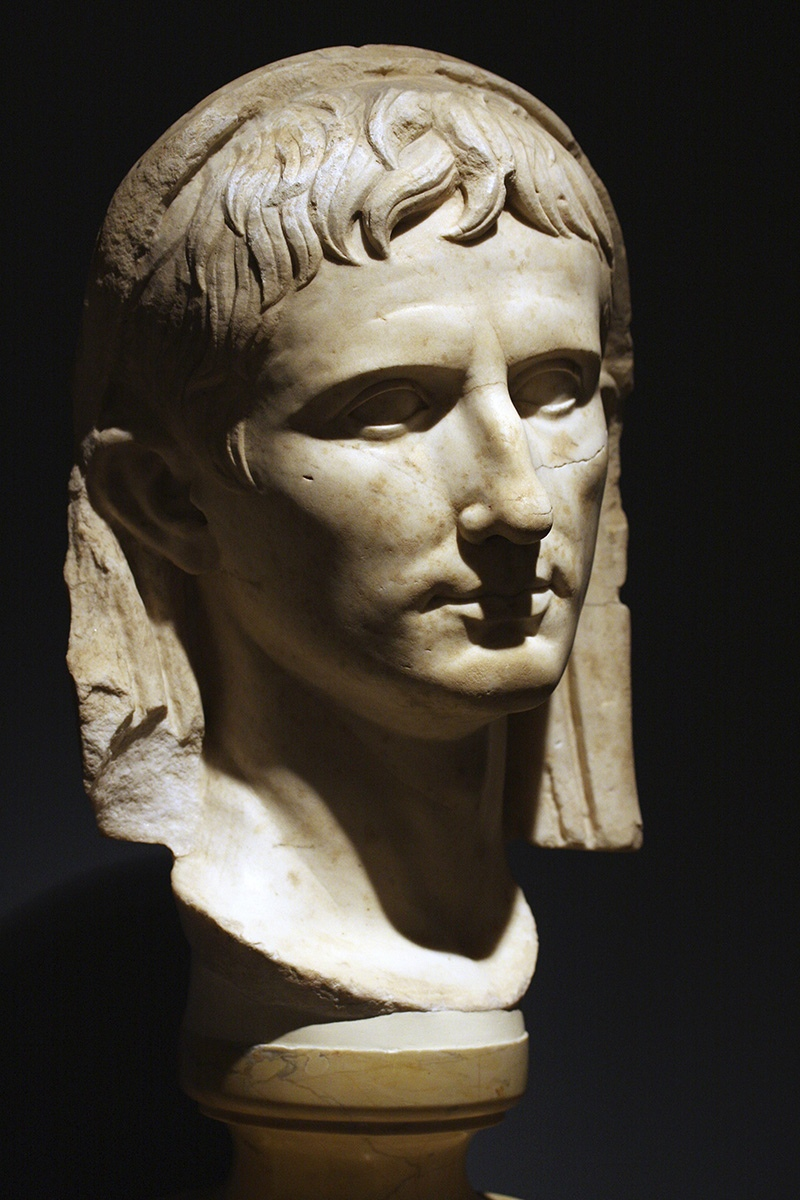
\includegraphics[scale=0.3]{VoprosOtvet/1585820685158259604.png}
	%	\label{fig:scipion} % Unique label used for referencing the figure in-text\end{document}
	%	%\addcontentsline{toc}{figure}{Figure \ref{fig:placeholder}} % Uncomment to add the figure to the table of contents%----------------------------------------------------------------------------------------
	\caption{Октавиан}%	CHAPTER 2
\end{figure}	

Коллега задал интересный вопрос, как так вышло, что после убийства Цезаря в последующем переделе власти наверх вылез Октавиан Август, сожрал всех остальных и получил абсолютную власть в Римском Мире. Кто он вообще такой, откуда вылез, как пробился и почему его не грохнули ещё в самом начале? Вот об этом, вкратце, я вам сегодня и поведаю.


Ху из Октавиан, этот загадочный племянник Цезаря? В самом вопросе и заключается ответ и на вопрос кто это и на вопрос как он выжил в те страшные годы. Он никто. Он пустота. И все его кажущиеся регалии это уже позднее натягивание бога и императора (кстати, в имперке был официальный культ гения императора, поэтому перед нами неиллюзорный бог-император ещё до того как это стало Вархаммером) на того пацана, который только начинал играть в Престолы.

А в те злополучные мартовские иды, когда сенаторы затыкали дядюшку ножами, а Марк Антоний в Народном Собрании размахивал окровавленной тогой Юлия - Октавиан пустота. Ему 14 или 15 лет, и он не успел вообще ничего. Есть мнение что пацан был любимчиком Цезаря, чуть ли не вторым сыном, но это последующая натяжка. Знаем мы то, что он был с Цезарем в Испании, точнее при нем, как и многие другие. Это абсолютно нормально: молодым патрициям положняк было покрутиться рядом когда взрослые делают Дела. И это единственная прямая протекция, да и её трудно назвать чем-то из ряда вон. В остальном в Риме происходил Цезарь, а где-то на третьем плане, абсолютно никак не вовлеченный ни во что значимое, происходил Октавиан. Пацану, ещё раз, лет пятнадцать, он даже для того времени совсем молодой.


Далее, есть мнение что раз он племяша Салата, значит имел право на свою долю пирога. Это неверно. Пересменка между двумя Триумвиратами и двумя же этапами римской гражданки это крушение всех и всяческих устоев в плане соблюдение традиций. Чем-то оная охлократия напоминала феерическое безумие Великой Французской Революции. Там уже глубоко не важно было кто ты по происхождению, патриции спокойненько записывались в плебеи и наоборот.

Решало, в конечном итоге, то, кто за тебя готов вписаться. Но и тут облом. Цезаря, если на список заговорщиков посмотреть, убивали не какие-то недобитые республиканцы, в вполне себе последовательные цезарианцы, в массе своей. Им не нужен был племяш Цезаря, они и так все его ближайшие соратники. Чуваки вроде Брута (есть мнение что он незаконнорожденный сын Салата, кстати) и Кассия скорее обеспечивали медийное сопровождение убийству, а ядро заговора это те люди, которые выигрывали Цезарю войну с галлаи, Помпеем, Катоном и вообще кем угодно. Им, крч, не надо было ничего особо доказывать, люди и так были при власти и при положении на момент когда случился "итыбрут". И племяша Цезаря, он там мог бы пригодиться, канешн, но не как самостоятельный игрок, а скорее как семья Александра Македонского, его гроб и прочие сашкины артефакты в тот момент, когда его наследники делили власть. Прост если у тебя больше таких штуковин, то ты трушный диадох. А если ты их все профукал при дележке и в более позднее время не нарулил, то, возможно, ты не трушный, не каноничный и вообще какой-то валенок. Люди могут отвернуться и уйти к кому покруче, предварительно отрезав те голову. Крч, сомнительная ценность родства с Цезарем в данном случае могла сыграть только вот так и больше никак.


Ну и, конечно, завещание. После того как Антоний помахал окровавленными тряпками покойного, и с большой неохотой не дал себя уговорить прям щас пойти на Палантин и поубивать там всех этих сенаторов к херам собачим, сами сенаторы притихли и призадумались. Общего праздника от смерти тирана как-то не выходило, никто шутку юмора не оценил и, крч, ситуация была сложная, как теперь власть удерживать в руках. В итоге договорились с Антонием на ратификацию не глядя всего цезарианского политического завещания, и как частного лица и как правителя государства. И на второе сел всё тот же Марк Антоний, получив в полное своё распоряжение бухгалтерию покойника, и право вытаскивать оттуда всякие документы и объявлять их волей покойного диктатора. Аргументируя это тем что "Юпитером клянусь, точно Цезарь лично писал и именно это и имел ввиду". То есть вы понимаете какая это была ульта, но выбора у сенаторов не было, так как Лепид, бессменный заместитель Цезаря по хозяйственным делам и проконсул Италии (ему лично подчинялись все легионы на сапоге) поддержал Антония.

Крч, Антонию Цезарь подарил своей смертью войска и право клепать чуть ли не любые законы от своего имени. Что же подарил племяннику столь же значимого? А ничего не подарил. Вот вообще. Октавиан как был ноль до смерти Юлия, так и остался им после неё, только теперь уже вроде как навсегда. Весь политический актив достался Антонию, а Октавиан свою долю от Цезаря получил как от частного лица, деньгами. Да, Юлий был сказочно богат, не без этого, и на Октавиана свалилось единомоментно реально очень много денег. Но они не были подкреплены ничем более значимым. И тот же Антоний мог бы их потом походя забрать "ради нашего великого дела", и распоряжаться как ему вздумается. Кстати, с шансами это было в планах, есть косвенные признаки. Крч, пацану казалось бы кирдык, сейчас его обезжирят и либо грохнут, либо посадят куда-нибудь на видное место и скажут "сиди вот сюда, заткнись, кивай и подписывай че дают", что тоже такая себе перспектива.


И вот тут ключевой момент Одиссеи. Пацан не сплоховал. Цезарь незадолго до своего убийства проводил достаточно ощутимые чистки в армии, перестраивая её на мирные рельсы и расселяя своих ветеранов. Вот им, собственно, Октавиан свои деньги и раздал, заодно призвав их на сверхсрочную службу. Не себе, естественно, а во блага Республики и под контролем Сената. А сам стал управлять этой античной ЧВК. Тем самым он лишился опасных денег, которые у него обязательно бы отняли, и снова стал никем, но уже с пачкой цезарианских ветеранов под рукой. Далее он нет, не лезет в политику, размахивать кровавыми тогами, читать филиппики - не про Октавиана. Октавиан, заимев первых лояльных людей с потрохами сдает себя сенатской партии, и цезарианских абсолютно аполитичных ветеранов подтаскивает за собой. А время, я напомню, страшное, каждый человек с войсками норовит в свою игру сыграть по любому поводу, поэтому эта подчеркнутая лояльность и аполитичность оценивается по достоинству, Октавиану дают расти и заниматься своими делами. Никакой политики, служим Республике, примус починяем.


А кровавая каша тем временем продолжает набирать обороты. Антонию откровенно сносит башку, он орет "АБСОЛЮТНАЯ ВЛАСТЬ!!!111", и начинает феерически быстро катить Рим к очередной гражданской войне. В конце концов так и вышло, довыпендривался Марк, объявил его Сенат "Врагом Республики" и послал армию мозги вправлять. Причем и тут Октавиан тихо так, незаметненько, сидит, с ветеранами Цезаря возится себе. Все пожилые сенаторы смотрят и умиляются, "какая молодежь пошла воспитанная!" думают. Крч, собрались сенаторы решать вопрос с Антонием, и Октавиана тож подтянули, за кампанию. Он там выставлял толи четверть армии, толи даж меньше, не помню. Ну и идут они, значит, Антония разбивать на север, и разбивают. В двух сражениях наносят ему два болезненных поражения и загоняют в казалось бы безвыходное положение...


*Вот теперь читайте внимательно!*


... но как-то так вышло, что оба консула, которые командовали сенатской армией в обоих битвах, они в них... ээээ.... умирают, один в первом бою, второй во втором. Какая неприятность-то, хех. И, я полагаю, не только они умирают, также под нож в пылу битвы идут слишком лояльные Сенату старшие офицеры, а в самой битве на убой бросаются самые боеспособные сенатские войска и стачиваются об Антония. А ребята Октавиана примус починяют и особых потерь не несут. А потом... набрали в грудь воздуха? Щас смешно будет. Так уот, а потом армия, а точнее то что от неё осталось, как-то сама собой переходит полностью в руки Октавиана, и он, загнав Антония в угол... объединяет с ним силы. Просто ставит старика перед фактом, мол, либо я сейчас, как пай-мальчик, размазываю твои войска по этим предгорьям, а твою башку везу в Рим, либо пошли со мной Рим брать. Его кто только не брал за последние годы, со времен Суллы больше десяти раз точно. Только уже нормально берем, и вычищаем там вообще всех кто хотя бы чисто теоретически способен мешать работать.


Вот такой вот пай-мальчик. Сидел там, глазки строил, ручки заламывал, потом прошвырнул вообще всех и сейчас во главе объединенной армии идет на Рим. Таким был, Октавиан Август в начале своей политической карьеры. Надул и Антония, когда деньги не дал забрать а на них себе армию личную запилил, де-факто, и в Сенате до кучи легализовался неплохо так. Причем многие пошли к Октавиану не томушта он "племяша", запомните, а томушта он "не Антоний". Антоний был редкостная мразь, чисто по личностным качествам, и ставить на него многим было не по нутру. А тут пацан, сразу видно что ушлый и далеко пойдет. Нарулив денег и сумев их удержать а потом использовать, Октавиан прошел этакий своеобразный "тест Тьюринга", показав что он не мебель или пешка, а тоже игрок в Престолы, и для него тоже хаос это лестница, так сказать. После этого он, оставаясь всё тем же лапочкой-зайчиком, последовательно вел ситуацию к войне и подливая масла в конфликт Антония с Сенатом, при этом оставаясь в стороне. Потом он озаботился получением контроля над армией, а дальше вы видели, разворот на 180 градусов и взятие Рима Октавианом, Антонием и присоединившимся к ним Лепидом, начало Второго Триумвирата. "Ведь это военная классика, похныкать о собственной слабости, затем мгновенно напасть и вы**ать оппонента в пасть", как пел ДЖ.


Вот так куется величие, господа. И из пустоты в годы потрясений вылупляются столь милые чудовища. Ну а раскрылся как чудовище Октавиан буквально не отходя от кассы, ещё до взятия Города, когда продумал и согласовал с коллегами по Второму Триумвирату проскрипционные списки, по сравнению с которыми Сулла просто образец милосердия и умеренности. Если после Суллы поговаривали что "стены можно было красить кровью", то после Октавиана с товарищами, я полагаю, можно было плавать текущим по улицам рекам крови на биремах и устраивать потешные морские сражения. Спокойное, расчетливое, планомерное истребление всех, кто, по мнению Октавиана, не вписывался в то будущее, которое он создавал. Очень хорошо организованный системный террор, где не брали пленных, никого не прощали и не договаривались. И он архитектор всего этого, он сам себя создал, сам себе все подчинил. И теперь в ручном режиме управлял процессом окончательного решения республиканского вопроса. Есть мнение что даже Антоний от происходящего нервничал немножечко, и смущался. Например, через жену Антония Октавиан подбил того на публичную расправу над Цицероном. Антоний его хотел просто убить чтоб тот наконец заткнулся, Октавиан настоял что убить мало, надо отрубить руки и язык, и прибить к дверям Капитолия. Чтобы помнили. Своих благодетелей раннего этапа, которые с него умилялись и давали играть в солдатиков он, конечно же, тоже пустил на дымящийся фарш. Деды думали противопоставить неуправляемому Антонию этого приличного, хорошо воспитанного и вежливого человека, ахаха. А он уже тогда подмечал для себя кого и как он убьет, потому что им не было места в том будущем, которое собирался подарить римскому миру Октавиан Август.


И знаете что самое интересное? Он ведь подарил его. Мир и безопасность Империи. На долгие 50 лет, от разгрома Антония и Клеопатры в Греции и до собственной смерти от банальной старости. Он чудовище из пустоты, плоть от плоти дитя той безумной эпохи, но он победил, и вошел в историю не вышеописанным кровавым адом, а тем, что все это было не зря. И если и есть где-то в истории пример оправданного тотального насилия, то вот он.


Такие дела, малята. 